\section{UC07 - Visualizzazione lista ticket di guasto}\label{uc:07}
\paragraph{Intenzione in contesto} L'attore primario desidera la lista dei ticket di guasto presenti nel sistema.

\paragraph{Attore primario} L'attore primario è o l'utente gestore o l'utente manutentore.
\paragraph{Precondizioni} L'attore primario è autenticato ed autorizzato dal sistema.
\paragraph{Post-condizioni} L'attore primario visualizza la lista dei ticket di guasto.
\paragraph{Scenario principale}
\begin{enumerate}
    \item L'attore primario richiede al sistema la lista dei ticket di guasto;
    \item la lista è stata visualizzata.
\end{enumerate}

\begin{figure}[h]
    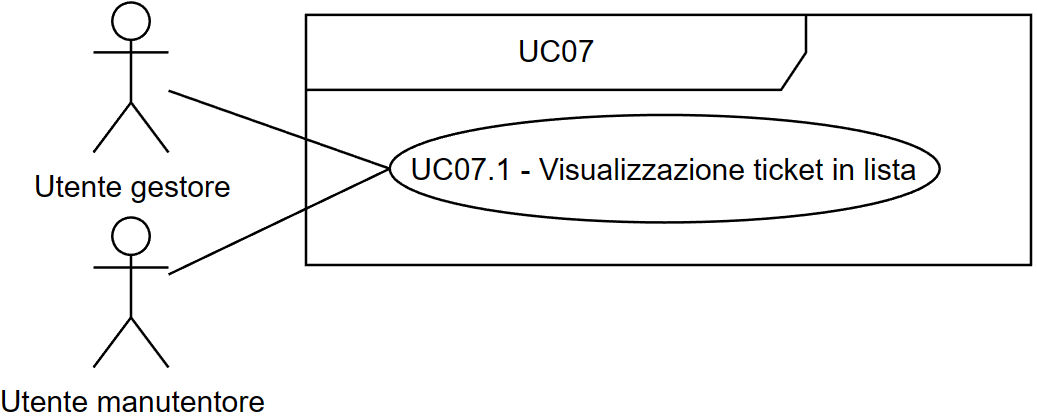
\includegraphics[width=\textwidth]{contenuti/img/casi_uso_grafici-uc07.png}
    \caption{UC7 in dettaglio}
    \label{fig:uc07}
\end{figure}

\subsection{UC07.1 - Visualizzazione ticket in lista}\label{uc:07.1}
\paragraph{Intenzione in contesto} L'attore primario vuole visualizzare il singolo ticket parte della lista.
\paragraph{Attore primario} L'attore primario è o l'utente gestore o l'utente manutentore.
\paragraph{Precondizioni} L'attore primario è autenticato ed autorizzato dal sistema.
\paragraph{Post-condizioni} L'attore primario visualizza il singolo ticket.
\paragraph{Scenario principale}
\begin{enumerate}
    \item L'attore primario richiede al sistema di visualizzare il singolo ticket in lista;
    \item il ticket è stato visualizzato.
\end{enumerate}

\begin{figure}[h]
    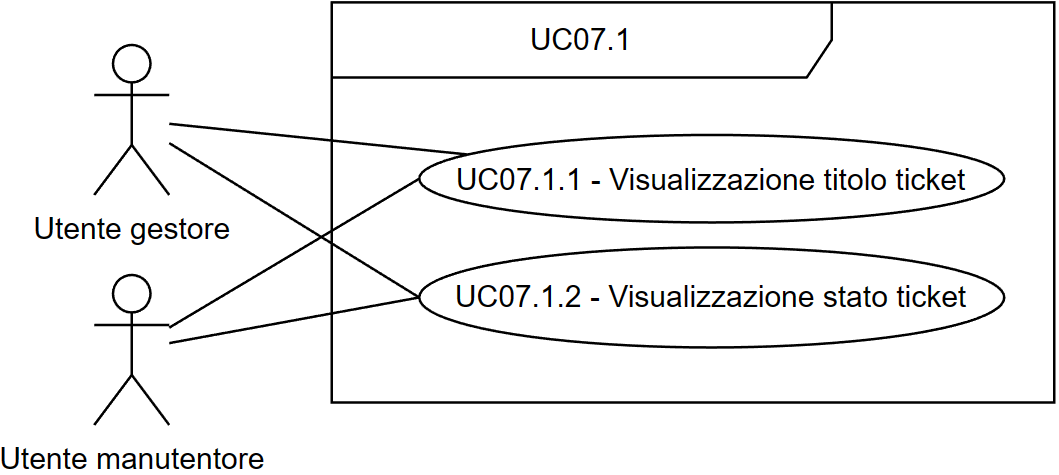
\includegraphics[width=\textwidth]{contenuti/img/casi_uso_grafici-uc07.1.png}
    \caption{UC07.1 in dettaglio}
    \label{fig:uc07.1}
\end{figure}

\subsection{UC07.1.1 - Visualizzazione titolo ticket}\label{uc:07.1.1}

\paragraph{Intenzione in contesto} L'attore primario vuole visualizzare il titolo del ticket;
\paragraph{Attore primario} L'attore primario è o l'utente gestore manutentore.
\paragraph{Precondizioni} L'attore primario è autenticato ed autorizzato dal sistema.
\paragraph{Post-condizioni} L'attore primario visualizza il titolo del ticket.
\paragraph{Scenario principale}
\begin{enumerate}
    \item L'attore primario richiede al sistema di visualizzare il titolo del ticket;
    \item il titolo del ticket è stato visualizzato.
\end{enumerate}

\subsection{UC07.1.2 - Visualizzazione stato ticket}\label{uc:07.1.2}

\paragraph{Intenzione in contesto} L'attore primario vuole visualizzare lo stato del ticket;
\paragraph{Attore primario} L'attore primario è o l'utente gestore manutentore.
\paragraph{Precondizioni} L'attore primario è autenticato ed autorizzato dal sistema.
\paragraph{Post-condizioni} L'attore primario visualizza lo stato del ticket.
\paragraph{Scenario principale}
\begin{enumerate}
    \item L'attore primario richiede al sistema di visualizzare lo stato del ticket;
    \item lo stato del ticket è stato visualizzato.
\end{enumerate}